% ========================================
%	Header einbinden
% ========================================

\documentclass[bibtotoc,titlepage]{scrartcl}

% Deutsche Spracheinstellungen
\usepackage[ngerman,german]{babel, varioref}
\usepackage[T1]{fontenc}
\usepackage[utf8]{inputenc}

%\usepackage{marvosym}

\usepackage{amsfonts}
\usepackage{amssymb}
\usepackage{amsmath}
\usepackage{amscd}
\usepackage{amstext}
\usepackage{float}
\usepackage{caption}
\usepackage{wrapfig}
\usepackage{setspace}
\usepackage{threeparttable}
\usepackage{footnote}

\usepackage{caption}
\usepackage{subcaption}

\newfloat{formel}{htbp}{for}
\floatname{formel}{Formel}


\usepackage{longtable}

%\usepackage{bibgerm}

\usepackage{footnpag}

\usepackage{ifthen}                 %%% package for conditionals in TeX
\usepackage{siunitx}
%Fr textumflossene Bilder und Tablellen
%\usepackage{floatflt} - veraltet

%Fr Testzwecke aktivieren, zeigt labels und refs im Text an.
%\usepackage{showkeys}

% Abstand zwischen zwei Abs�zen nach DIN (1,5 Zeilen)
% \setlength{\parskip}{1.5ex plus0.5ex minus0.5ex}

% Einrckung am Anfang eines neuen Absatzes nach DIN (keine)
%\setlength{\parindent}{0pt}

% R�der definieren
% \setlength{\oddsidemargin}{0.3cm}
% \setlength{\textwidth}{15.6cm}

% bessere Bildunterschriften
%\usepackage[center]{caption2}


% Probleml�ungen beim Umgang mit Gleitumgebungen
\usepackage{float}

% Nummeriert bis zur Strukturstufe 3 (also <section>, <subsection> und <subsubsection>)
%\setcounter{secnumdepth}{3}

% Fhrt das Inhaltsverzeichnis bis zur Strukturstufe 3
%\setcounter{tocdepth}{3}

\usepackage{exscale}

\newenvironment{dsm} {\begin{displaymath}} {\end{displaymath}}
\newenvironment{vars} {\begin{center}\scriptsize} {\normalsize \end{center}}


\newcommand {\en} {\varepsilon_0}               % Epsilon-Null aus der Elektrodynamik
\newcommand {\lap} {\; \mathbf{\Delta}}         % Laplace-Operator
\newcommand {\R} { \mathbb{R} }                 % Menge der reellen Zahlen
\newcommand {\e} { \ \mathbf{e} }               % Eulersche Zahl
\renewcommand {\i} { \mathbf{i} }               % komplexe Zahl i
\newcommand {\N} { \mathbb{N} }                 % Menge der nat. Zahlen
\newcommand {\C} { \mathbb{C} }                 % Menge der kompl. Zahlen
\newcommand {\Z} { \mathbb{Z} }                 % Menge der kompl. Zahlen
\newcommand {\limi}[1]{\lim_{#1 \rightarrow \infty}} % Limes unendlich
\newcommand {\sumi}[1]{\sum_{#1=0}^\infty}
\newcommand {\rot} {\; \mathrm{rot} \,}         % Rotation
\newcommand {\grad} {\; \mathrm{grad} \,}       % Gradient
\newcommand {\dive} {\; \mathrm{div} \,}        % Divergenz
\newcommand {\dx} {\; \mathrm{d} }              % Differential d
\newcommand {\cotanh} {\; \mathrm{cotanh} \,}   %Cotangenshyperbolicus
\newcommand {\asinh} {\; \mathrm{areasinh} \,}  %Area-Sinus-Hyp.
\newcommand {\acosh} {\; \mathrm{areacosh} \,}  %Area-Cosinus-H.
\newcommand {\atanh} {\; \mathrm{areatanh} \,}  %Area Tangens-H.
\newcommand {\acoth} {\; \mathrm{areacoth} \,}  % Area-cotangens
\newcommand {\Sp} {\; \mathrm{Sp} \,}
\newcommand {\mbe} {\stackrel{\text{!}}{=}}     %Must Be Equal
\newcommand{\qed} { \hfill $\square$\\}
\renewcommand{\i} {\imath}
\def\captionsngerman{\def\figurename{\textbf{Abb.}}}

%%%%%%%%%%%%%%%%%%%%%%%%%%%%%%%%%%%%%%%%%%%%%%%%%%%%%%%%%%%%%%%%%%%%%%%%%%%%
% SWITCH FOR PDFLATEX or LATEX
%%%%%%%%%%%%%%%%%%%%%%%%%%%%%%%%%%%%%%%%%%%%%%%%%%%%%%%%%%%%%%%%%%%%%%%%%%%%
%%%
\ifx\pdfoutput\undefined %%%%%%%%%%%%%%%%%%%%%%%%%%%%%%%%%%%%%%%%% LATEX %%%
%%%
\usepackage[dvips]{graphicx}       %%% graphics for dvips
\DeclareGraphicsExtensions{.eps,.ps}   %%% standard extension for included graphics
\usepackage[ps2pdf]{thumbpdf}      %%% thumbnails for ps2pdf
\usepackage[ps2pdf,                %%% hyper-references for ps2pdf
bookmarks=true,%                   %%% generate bookmarks ...
bookmarksnumbered=true,%           %%% ... with numbers
hypertexnames=false,%              %%% needed for correct links to figures !!!
breaklinks=true,%                  %%% breaks lines, but links are very small
linkbordercolor={0 0 1},%          %%% blue frames around links
pdfborder={0 0 112.0}]{hyperref}%  %%% border-width of frames
%                                      will be multiplied with 0.009 by ps2pdf
%
%\hypersetup{ pdfauthor   = {Hannes Franke; Julius Tilly},
%pdftitle    = {x}, pdfsubject  = {Protokoll FP}, pdfkeywords = {V301, Innenwiderstand, Leistungsanpassung},
%pdfcreator  = {LaTeX with hyperref package}, pdfproducer = {dvips
%+ ps2pdf} }
%%%
\else %%%%%%%%%%%%%%%%%%%%%%%%%%%%%%%%%%%%%%%%%%%%%%%%%%%%%%%%%% PDFLATEX %%%
%%%
\usepackage[pdftex]{graphicx}      %%% graphics for pdfLaTeX
\DeclareGraphicsExtensions{.pdf}   %%% standard extension for included graphics
\usepackage[pdftex]{thumbpdf}      %%% thumbnails for pdflatex
\usepackage[pdftex,                %%% hyper-references for pdflatex
bookmarks=true,%                   %%% generate bookmarks ...
bookmarksnumbered=true,%           %%% ... with numbers
hypertexnames=false,%              %%% needed for correct links to figures !!!
breaklinks=true,%                  %%% break links if exceeding a single line
linkbordercolor={0 0 1},
linktocpage]{hyperref} %%% blue frames around links
%                                  %%% pdfborder={0 0 1} is the default
% \hypersetup{
% pdftitle    = {V301 Innenwiderstand und Leistungsanpassung}, 
% pdfsubject  = {Protokoll AP}, 
% pdfkeywords = {V301, Innenwiderstand, Leistungsanpassung},
% pdfsubject  = {Protokoll AP},
% pdfkeywords = {V301, Innenwiderstand, Leistungsanpassung}}
%                                  %%% pdfcreator, pdfproducer,
%                                      and CreationDate are automatically set
%                                      by pdflatex !!!
\pdfadjustspacing=1                %%% force LaTeX-like character spacing
\usepackage{epstopdf}
%
\fi %%%%%%%%%%%%%%%%%%%%%%%%%%%%%%%%%%%%%%%%%%%%%%%%%%% END OF CONDITION %%%
%%%%%%%%%%%%%%%%%%%%%%%%%%%%%%%%%%%%%%%%%%%%%%%%%%%%%%%%%%%%%%%%%%%%%%%%%%%%
% seitliche Tabellen und Abbildungen
%\usepackage{rotating}
\usepackage{ae}
\usepackage{
  array,
  booktabs,
  dcolumn
}
\makeatletter 
  \renewenvironment{figure}[1][] {% 
    \ifthenelse{\equal{#1}{}}{% 
      \@float{figure} 
    }{% 
      \@float{figure}[#1]% 
    }% 
    \centering 
  }{% 
    \end@float 
  } 
  \makeatother 


  \makeatletter 
  \renewenvironment{table}[1][] {% 
    \ifthenelse{\equal{#1}{}}{% 
      \@float{table} 
    }{% 
      \@float{table}[#1]% 
    }% 
    \centering 
  }{% 
    \end@float 
  } 
  \makeatother 
%\usepackage{listings}
%\lstloadlanguages{[Visual]Basic}
%\allowdisplaybreaks[1]
%\usepackage{hycap}
%\usepackage{fancyunits}

% ========================================
%	Angaben für das Titelblatt
% ========================================

\title{Lehrstuhlversuch E1 - Röntgenreflektometrie\\				% Titel des Versuchs 
\large TU Dortmund, Fakultät Physik\\ 
\normalsize Fortgeschrittenen-Praktikum}

\author{Jan Adam\\			% Name Praktikumspartner A
{\small \href{jan.adam@tu-dortmund.de}{jan.adam@tu-dortmund.de}}	% Erzeugt interaktiven einen Link
\and						% um einen weiteren Author hinzuzfügen
Dimitrios Skodras\\					% Name Praktikumspartner B
{\small \href{dimitrios.skodras@tu-dortmund.de}{dimitrios.skodras@tu-dortmund.de}}		% Erzeugt interaktiven einen Link
}
\date{09.06.2015}				% Das Datum der Versuchsdurchführung

% ========================================
%	Das Dokument beginnt
% ========================================

\begin{document}

% ========================================
%	Titelblatt erzeugen
% ========================================

\maketitle					% Jetzt wird die Titelseite erzeugt
\thispagestyle{empty} 				% Weder Kopfzeile noch Fußzeile

% ========================================
%	Der Vorspann
% ========================================

%\newpage					% Wenn Verzeichnisse auf einer neuen Seite beginnen sollen
%\pagestyle{empty}				% Weder Kopf- noch Fußzeile für Verzeichnisse

\tableofcontents

%\newpage					% eine neue Seite
%\thispagestyle{empty}				% Weder Kopf- noch Fußzeile für Verzeichnisse
%\listoffigures					% Abbildungsverzeichnis

%\newpage					% eine neue Seite
%\thispagestyle{empty}				% Weder Kopf- noch Fußzeile für Verzeichnisse
%\listoftables					% Tabellenverzeichnis
\newpage					% eine neue Seite


% ========================================
%	Kapitel
% ========================================

%\section{Einleitung}				% Bei Bedarf

\section{Theorie}
\subsection{Fresnelsche Formeln}
Die Fresnelformeln geben den Reflexions- (R) und den Transmissionsgrad (T) von EM-Wellen an der Grenzfläche zweier Medien mit Brechungsindizes $n_1$ und $n_2$ an.
Entsprechend der beiden Polarisationsrichtungen (senkrecht und parallel) gibt es vier verschiedene Formeln
\begin{align}
 T_s &= \frac{2n_1}{n_1 \cos\alpha + n_2\cos\beta}\\
 R_s &= \frac{n_1 \cos\alpha - n_2\cos\beta}{n_1 \cos\alpha + n_2\cos\beta}\\
 T_p &= \frac{2n_1}{n_2 \cos\alpha + n_1\cos\beta}\\
 R_p &= \frac{n_2 \cos\alpha - n_1\cos\beta}{n_2 \cos\alpha + n_1\cos\beta},
\end{align}
\noindent mit $\alpha$ als Winkel zwischen einfallendem Stahl und Lot und $\beta$ als Winkel zwischen ausfallendem Stahl und Lot. Das Lorentz-Modell erklärt,
dass Materie für Röntgenstrahlung einen Brechungsindex $n = 1-\delta + \text{i}\beta$ aufweist. Hierin lautet die dielektrische Funktion
\noindent mit $\alpha$ als Winkel zwischen einfallendem Strahl und Lot und $\beta$ als Winkel zwischen ausfallendem Strahl und Lot. Das Lorentz-Modell erklärt,
dass Materie für Röntgenstrahlung einen Brechungsindex $n = 1-\delta <1$ aufweist. Hierin lautet die dielektrische Funktion
\begin{align}
 \epsilon(\omega) = 1 + \frac{4\pi n_0 e^2}{m_\text{e}} \sum\limits_i \frac{f_i}{\omega_i^2 - \omega^2 - \text{i}\omega\Gamma_i},
\end{align}
für Materialien mit $Z=\sum_i f_i$ Elektronen pro Atom mit $i$ unterschiedlichen Eigenfrequenzen $\omega_i$ und Dämpfungen $\Gamma_i$. $n$ erhält man als
Realteil von $\sqrt{\epsilon}$ und lautet $f_i / \omega_i^2 - \omega^2$. Der Imaginärteil $\beta$ beschreibt die Abschwächung der Amplitude im Medium.
Der Realteil wird für Röntgenstrahlung ($\omega_i >\omega$) positiv und $\text{Re}(n)<1$, was
unterhalb eines kritischen Winkels $\alpha_c\approx \sqrt{2\delta}=\lambda\sqrt{r_\text{e}\rho /\pi}$ an der Grenzfläche zur Totalreflexion führt, mit
der Wellenlänge $\lambda$, der Elektronendichte im Material $\rho$ und dem klassischen Elektronenradius $r_\text{e}$. Die Abweichung $\delta$ ist 
$\mathcal{O}(10^{-6})$, sodass 
$n_1 \approx n_2 \approx 1$ genähert wird und Polarisationen nicht mehr unterschieden werden. Hiermit wird die Gesamtreflektivität $R_F = |R_{s,p}|^2$ für
große Winkel zu
\begin{align}
 R_F \approx \left(\frac{\alpha_c}{\alpha_i}\right)^4.
\end{align}

\subsection{Zweischichtsystem}
Kiessing-Ringe sind Modulationen der Reflexionskurve, hervorgerufen durch Interferenz der reflektierten Strahlung. Die Minima entstehen, wenn der 
Phasenunterschied gerade ein ungerades Vielfaches der Wellenlänge $\lambda$ ist. Ziel hier ist eine Beziehung zwischen der Winkeldifferenz zweier Kiessing-Minima 
in Beziehung zur Schichtdicke $d$ zu setzen. Der Gangunterschied ist ein ungeradzahliges Vielfaches der halben Wellenlänge und liest sich
\begin{align}
 \Delta l_i = 2 d \sin\alpha_i = \frac{2n+1}{2}\lambda.
\end{align}
Die Gangunterschieddifferenz ist daher
\begin{align}
 \Delta l_i -\Delta l_{n-1}= 2 d \sin\alpha_i - 2d\sin\alpha_{i-1} \approx 2d (\alpha_i - \alpha_{i-1})
\end{align}
mit der Annahme kleiner Winkel ($\sin\alpha \approx \alpha$).  , was zur
gesuchten Relation führt
\begin{align}
 d \approx \frac{\lambda}{2\Delta\alpha_i} = \frac{2\pi}{\Delta q_z},
\end{align}
mit $\vec q = \vec k_\text{f} - \vec k_\text{i}$ als Wellenvektorübertrag mit der $z$-Komponente $q_z = 2k\sin(\alpha_i)$ und $\Delta q_z$ als die Differenz dieser 
Komponente an den Minima.

\subsection{Parratt-Algorithmus}
Bei mehreren Schichten wird die Reflektivität durch Überlagerung unterschiedlicher Brechungsindizes komplizierter. Hierzu wird der Paratt-Algorithmus als
rekursive Lösung verwandt. Mit der Fresnelreflektivität $r_{j,j+1} = \frac{k_{z,j}-k_{z,j+1}}{k_{z,j}+k_{z,j+1}}$ an der Grenzfläche $j$ und der $z$-Komponente 
des Wellenvektors $k_{z,j} = k\sqrt{n_j^2-\cos^2\alpha_i}$
lautet das Amplitudenverhältnis nach dem Algorithmus
\begin{align}
 X_j = \frac{R_j}{T_j} = \text{e}^{-2ik_{z,j}z_j}\frac{r_{j,j+1} + X_{j+1} \text{e}^{+2ik_{z,j}z_j}}{1 + r_{j,j+1} X_{j+1}\text{e}^{+2ik_{z,j}z_j}}.
\end{align}
Angewandt auf ein System mit $N=2$ Schichten mit unendlich dickem Vakuum und Substrat. Somit gilt als Startwert $X_3 = 0$ und damit für die beiden weiteren
\begin{align}
 X_2 &= r_{2,3}\text{e}^{-2ik_{z,2}z_2}\\
 X_1 &= \frac{r_{1,2}+\text{e}^{-2ik_{z,2}z_2}}{1+r_{1,2}\text{e}^{-2ik_{z,2}z_2}}.
\end{align}
Mit \texttt{Python} lässt sich die Reflektivität graphisch (Abbildung \ref{pic_ReflNormal}) darstellen.

\begin{figure}[H]
 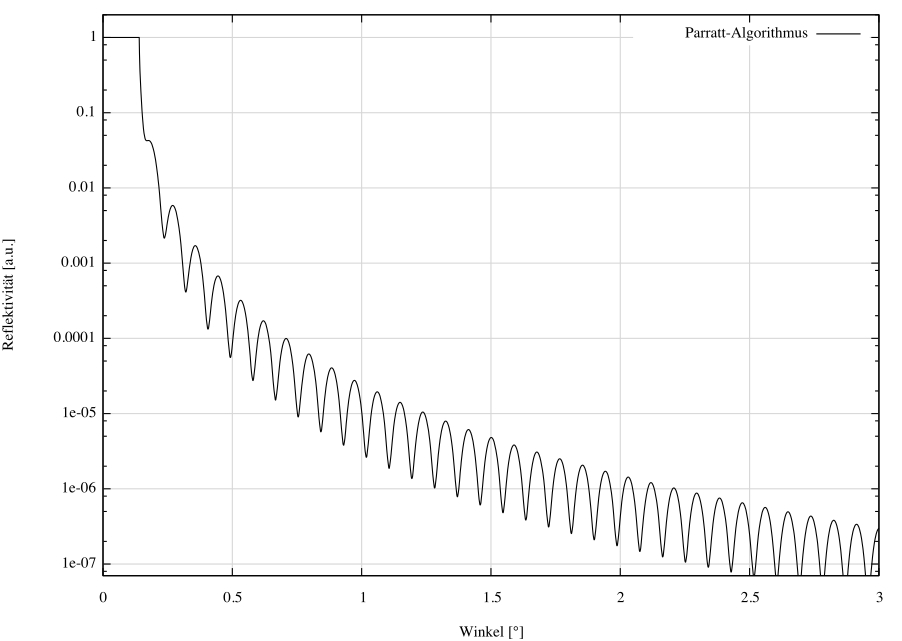
\includegraphics[width=\textwidth]{../pics/normal.jpg}
 \caption{Reflektivität mit dünner Schicht ($500$ $\mathring{A}$) und unendlich dickem Substrat, ermittelt durch den Parratt-Algorithmus}
 \label{pic_ReflNormal}
\end{figure}
\noindent
Erweitern lässt sich dieses System noch um die Rauigkeit $\sigma$, was zu den modifizierten Fresnelformeln führt
\begin{align}
 r^\sigma_{j,j+1} = r_{j,j+1} \cdot \text{e}^{-2k_{z,j}k_{z,j+1}\sigma_j^2}.
\end{align}
Mit einem $\sigma = 6\mathring{A}$ und sonst identischen Parametern verändert sich die Kurve so, wie in Abbildung \ref{pic_ReflRau} gezeigt. Die Kurve fällt aufgrund
der Rauigkeit deutlich schneller ab.

\begin{figure}[H]
 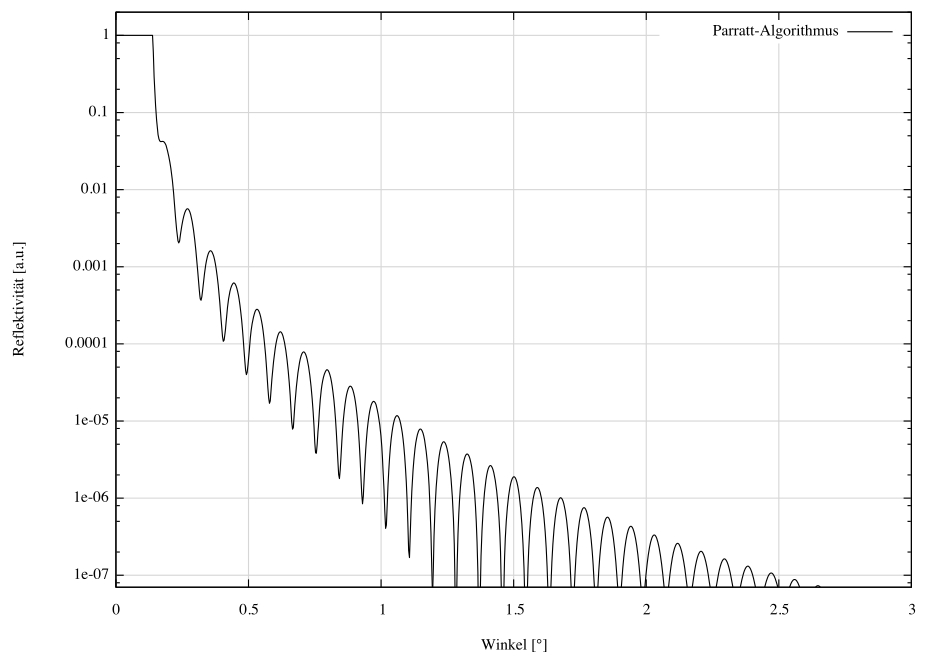
\includegraphics[width=\textwidth]{../pics/rau.jpg}
 \caption{Reflektivität mit dünner Schicht ($500$ $\mathring{A}$) und unendlich dickem Substrat, ermittelt durch den Parratt-Algorithmus. Die Rauigkeit des Substrats ist berücksichtigt}
 \label{pic_ReflRau}
\end{figure}


\section{Durchführung}
\subsection{Das D8-Labordiffraktometer}
Die Messungen werden an einem D8-Labordiffraktometer (auch $\theta - \theta$-Diffraktometer) durchgeführt. Die Röntgenstrahlung kommt von einer 
Kupferanodenröhre, wird wird von mehreren parabolischen Spiegeln gebündelt und monochromatisiert, sodass der austretende Strahl eine Wellenlänge von
$\lambda = 1.54 \AA$ und eine Intensität von $10-100$ s$^{-1}$m$^{-2}$ hat. Ein Autoabsorber schwächt die Intensität bei hohen Zählraten und eine Blende
blockiert unerwünschte Streustahlung ausgehend von der Reflexion an der Probenoberfläche. Nach einer weiteren Blende folgt der Eintritt in den NaI(TI)-Detektor.
\subsection{Probenjustage und Programm}
\textbf{1.}\\
Die Probe wird in das Diffraktometer zwischen Röhre und Detektor gelegt. Über Schrittmotoren lässt sich die Position in alle Raumrichtungen verschieben.\\
\textbf{2.}\\
Nun wird ein Detectorscan durchgeführt, bei dem die Röhre fix und der Detektor ohne Probe dazwischen bewegt wird. Aufgenommen wird das Intensitätmaximum
bei einem gewissen Winkel, bei dem beide Bestandteile sich auf einer Achse befinden.
\\ \textbf{3.}\\
Die Probe liegt so, dass sie die halbe Intensität des Primärstrahls abschattet. Der Z-Scan ermittelt die $z$-Komponente, bei der dies der Fall ist.
\\ \textbf{4.}\\
Detektor und Röhre werden nun um denselben Winkel (zwischen $\pm1^\circ$ um die 0) gedreht, sodass sie sich permanenet gegenüber stehen. Idealerweise ergibt
sich ein symmetrisches Dreieck in der Intensität bezüglich des Winkels. Die Breite des Dreiecks dient zur Auswertung des Geometriewinkels, bei dem der Strahl
die gesamte Probenoberfläche abdeckt. Dieser Prozess wird Rockingscan genannt.
\\ \textbf{5.}\\
Die Schritte 3. und 4. sind ggf. zu wiederholen, bis die $z$-Kompenente zur halben Intensität führt und das Intensitätsdreieck symmetrisch ist.
\\ \textbf{6.}\\
Detektor und Röhre werden etwas aus ihrer gemeinsamen Achse gedreht, hier also $2\theta = 0.3^\circ$ kleiner als der kritische Winkel $\alpha_c$ zur Totalreflexion.
Mit dieser Einstellung wird ein Rockingscan durchgeführt in einem Bereich von 0.1 und 0.2 wegen des zu erwartenden Maximums bei 0.15.
\\ \textbf{7.}\\
Ein erneuter Z-Scan unter $2\theta=0.3^\circ$ wird durchgeführt. Dieser dient der genaueren Feststellung des Maximums aus der Intensitätskurve. 
\\ \textbf{8.}\\
Beim Winkel $2\theta=1^\circ$ wird ein weiterer Rockingscan entsprechend 6. durchgeführt, jedoch um das erwartete Maximum bei 0.5.
\\ \textbf{9.}\\
Die Röntgenröhre ist nun an der richtigen Stelle bezüglich der größten Intensität, der Detektor ist jedoch nur relativ zur Röhre ausgerichtet, was auch heißt,
dass $\alpha_\text{i} \neq \alpha_\text{f}$ ist. Also wird ein weiterer Detectorscan nach 2. durchgeführt mit genullten Winkeln und herausgefahrener Probe.
\\ \textbf{10.}\\
Schließlich werden noch weitere Rockingscans bei verschiedenen Winkeln durchgeführt, um zu prüfen, ob die Beziehung $2\theta = 2\alpha_\text{i}$ oberhalb
und unterhalb des kritischen Winkels stimmt.%\vspace{0.2cm}
\\
\noindent
Als Scanbereich (Winkel) wird das Intervall $0^\circ$ bis 
$2.5^\circ$ mit einer Schrittweite von $0.0025^\circ$ gewählt. Pro Messung wird die Intensität über eine Zeitraum von $t=\SI{10}{\second}$ integriert. 
Um den Untergrund durch Streustrahlen zu unterdrücken, wird außerdem ein ``Diffuser Scan'' durchgeführt. Dabei wird die eben beschriebene Messung wiederholt,
der Detektor wird jedoch um $0.1^\circ$ bezüglich des Ausfallwinkels der Röntgenstrahlung verschoben. Dadurch wird nur nur die diffus gestreute 
Röntgenstrahlung gemessen, die bei der eigentlichen Messung als Untergrund eingeht. Durch Subtraktion beider Scans kann die Messung um den Untergrund 
korrigiert werden.

\section{Auswertung}
In diesem Versuch sollen Dispersion und Rauigkeit des Siliziumwafers, sowie die Schichtdicke, Dispersion und Rauigkeit der Polysterolschicht bestimmt werden.

% \begin{figure}[h]
% 	\centering
% 	\includegraphics[width=\textwidth]{../tex/bilder/data.pdf}
% 	\caption{Messwerte des Reflektivitätsscans und des diffusen Scans.}
% 	\label{pic:daten}
% \end{figure}

Abbildung \ref{pic:daten} zeigt die bei den Scans aufgenommenen Daten. Dargestellt sind die Reflektivitätsmessung sowie der "Diffuse Scan"\. Der Diffuse Scan wird vom Reflektivitätsscan subtrahiert.

Anschließend müssen die Daten um den Geometriefaktor $G$ korrigiert werden.
Der Geometriefaktor $G$ entspricht dem Anteil des Strahls, der die Fläche des Wafers trifft:
\begin{align}
	G &= \frac{D}{d_0}\cdot \sin(\alpha_i) &\text{für $\alpha_i < \alpha_g$}\\
	G &= 1 &\text{sonst}
\end{align}
 und somit in Richtung des Detektors reflektiert wird. Bei Winkeln $\alpha_i >$ Geometriewinkel $\alpha_g$, trifft immer der gesamte Strahl auf die Probe, daher gilt dort $G=1$. Bei kleineren Winkeln geht jedoch ein Teil des Lichts verloren, wodurch nur ein Teil des eigentlichen Signals im Detektor gemessen wird. Hier muss das Signal um den Geometriefaktor korrigiert werden.

Bei einem Strahldurchmesser von $D = \SI{0.1}{\milli\meter}$ und einer Probendicke von $d_0 = \SI{30}{\milli\meter}$ ergibt sich für den Geometriewinkel $\alpha_g$ ein Wert von
\begin{align}
	\alpha_\text{g} = \arcsin\left(\frac{d_0}{D}\right) = \SI{0.191}{\degree}.
\end{align}
Unterhalb dieses Winkels muss der Geometriefaktor bei der Auswertung berücksichtigt werden. In Abbildung \ref{pic:geometrie} sind sowohl die ursprüngliche Datenreihe, als auch die korrigierte Datenreihe eingetragen. Bei kleinen Winkeln beträgt die Korrektur mehr als eine Größenordnung.

% \begin{figure}[h]
% 	\centering
% 	\includegraphics[width=\textwidth]{../tex/bilder/geometriefaktor.pdf}
% 	\caption{Messwerte mit und ohne Korrektur durch den Geometriefaktor.}
% 	\label{pic:geometrie}
% \end{figure}


Um nun Dispersion und Rauigkeit des Siliziumwafers, sowie Schichtdicke, Dispersion und Rauigkeit der Polysterolschicht zu bestimmen, wird mittels Python ein Fit der aufgenommenen Messwerte durchgeführt. Der Brechungsindex der Luft wird dabei konstant als $n_1=1$ angenommen.

In Abbildung \ref{pic:fit} wurde neben den Datenpunkten zwei gefittete Kurven eingetragen. Die blaue Kurve ergibt sich durch die Parameter, die das Pythonscript errechnet hat:
\begin{align*}
	n_2 &= 1-2.8\cdot 10^{-6}\\
	n_3 &= 1-7.2\cdot 10^{-6}\\
	\sigma_1 &= 5.5\cdot 10^{-10}\,\si{\meter} \\
	\sigma_2 &= 2.4\cdot 10^{-10}\,\si{\meter}\\
	z_2&= 210.0\cdot 10^{-10}\,\si{\meter}
\end{align*}

Die blaue Kurve weicht jedoch um bis zu 30\% von den Messwerten ab. Daher wurden die angegebenen Parameter per Hand weiter optimiert, um eine bessere Abdeckung zu erzielen. Die neue Kurve wird in rot dargestellt.
% \begin{figure}[H]
% 	\centering
% 	\includegraphics[width=\textwidth]{../tex/bilder/fit.pdf}
% 	\caption{Korrigierte Messwerte und Theoriekurven.}
% 	\label{pic:fit}
% \end{figure}


Die rote Kurve ergibt sich durch folgende Parameterwahl:
\begin{align*}
n_2 &= 1-3.5\cdot 10^{-6}\\
n_3 &= 1-9.24\cdot 10^{-6}\\
\sigma_1 &= 4.78\cdot 10^{-10}\,\si{\meter} \\
\sigma_2 &= 3.28\cdot 10^{-10}\,\si{\meter}\\
 z_2&= 209.8\cdot 10^{-10}\,\si{\meter}
\end{align*}

Bei Durchführung des Fits ist es wichtig, darauf zu achten, dass der erste Peak bis ungefähr \SI{0.2}{\degree} nicht verwendet wird. Bei einem Winkel von $0^\circ < \alpha < 0.2^\circ$ trifft die Röntgenstrahlung so flach auf den Wafer, dass ein Teil von ihr den Wafer verfehlt und ohne Reflektion direkt in den Detektor trifft. Diese Werte dürfen daher nicht den Fit beeinflussen.

\section{Diskussion}
Es gelingt nicht, eine perfekte Übereinstimmung zwischen Messwerten und Theoriekurve zu erzielen.
Dies deutet darauf hin, dass die Struktur der untersuchte Probe vom Theoriemodell abweicht. In der Tat bildet sich durch den Sauerstoff aus der Luft auf der Siliziumschicht eine feine Oxidschicht, die im verwendeten Modell nicht berücksichtigt wurde.
Entsprechend gelingt es dem automatischen Fit nicht, die bestmöglichste Übereinstimmung zu finden.

Durch eine manuelle Optimierung kann die Theoriekurve den Messwerten weiter angenähert werden, eine sehr gute Übereinstimmung kann jedoch entweder nur im ersten Peak oder nur in den nachfolgenden Erreicht werden. Hier wurde ein Kompromiss aus beidem gewählt, um starke lokale Schwankungen zu vermeiden.

Beide Auswertungen gelangen zu einer ähnlichen Schichtdicke des Polysterols von etwa \SI{210}{\angstrom}.
Die Rauigkeit dieser Schicht variiert jedoch je nach Fit zwischen \SI{2.4}{\angstrom} und \SI{3.2}{\angstrom}, was ein Hinweis auf die vorhandene Oxidschicht sein kann.



\vspace{2cm}
\textbf{Literatur}

\vspace{0.3cm}
[1] Anleitung des Lehrstuhlversuchs

% ========================================
%	Literaturverzeichnis
% ========================================

%\bibliographystyle{plainnat}			% Bibliographie-Style auswählen
%\bibliography{BIBDATEI}			% Literaturverzeichnis

% ========================================
%	Das Dokument endent
% ========================================

\end{document}
